\documentclass[12pt]{Qual}
\usepackage{preamble}

\name{Kayla Orlinsky}
\course{Complex Analysis Exam}
\term{Spring 2012}
\hwnum{Spring 2012}

\begin{document}

\begin{problem} $\,$
Suppose $a>0$. Evaluate the integral $$\int_{-\infty}^\infty\frac{\sin(ax)}{x(x^2+1)}dx$$ be careful to justify your methods.
\end{problem}


\begin{solution}$\,$
We will use ``Ol' Faithful'' the contour around the upper half plane avoiding the origin.

\begin{center}
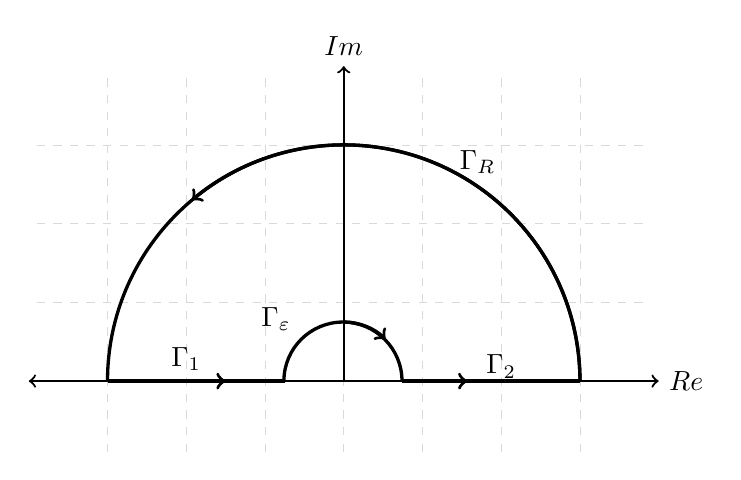
\begin{tikzpicture}
\draw[help lines, color=gray!30, dashed] (-3.9,-0.9) grid (3.9,3.9);
\draw[->,very thick] (3,0) arc (0:130:3cm);
\draw[very thick] (3,0) arc (0:180:3cm) node[above,yshift=2.5cm,xshift=4.7cm]{$\Gamma_R$};
\draw[->,very thick] (0,0.75) arc (90:45:0.75cm);
\draw[very thick] (0.74,0) arc (0:180:0.75cm) node[above,yshift=0.5cm,xshift=-0.1cm]{$\Gamma_\varepsilon$};
\draw[->,very thick] (0.74,0) -- (1.57,0);
\draw[very thick] (0.75,0) -- (3,0) node[above,yshift=-0.1cm,xshift=-1cm]{$\Gamma_2$};
\draw[->,very thick] (-3,0) -- (-1.5,0);
\draw[very thick] (-0.74,0) -- (-3,0) node[above,yshift=0cm,xshift=1cm]{$\Gamma_1$};
\draw[<->, thick] (-4,0)--(4,0) node[right]{$Re$};
\draw[->, thick] (0,0)--(0,4) node[above]{$Im$};
\end{tikzpicture}
\end{center}

Let \begin{align*}
    I_1&=\int_{\Gamma_1}\frac{e^{iaz}}{z(z^2+1)}dz\\
    I_2&=\int_{\Gamma_2}\frac{e^{iaz}}{z(z^2+1)}dz\\
    I_\varepsilon&=\int_{\Gamma_\varepsilon}\frac{e^{iaz}}{z(z^2+1)}dz\\
    I_R&=\int_{\Gamma_R}\frac{e^{iaz}}{z(z^2+1)}dz
\end{align*}

Now, \begin{align*}
    I_1+I_2&=\int_{-R}^{-\varepsilon}\frac{e^{iax}}{x(x^2+1)}dx+\int_\varepsilon^R\frac{e^{iax}}{x(x^2+1)}dx\\
    &=\int_R^\varepsilon\frac{-e^{-iax}}{-x((-x)^2+1)}dx+\int_\varepsilon^R\frac{e^{iax}}{x(x^2+1)}dx\\
    &=\int_\varepsilon^R\frac{-e^{-iax}}{x(x^2+1)}dx+\int_\varepsilon^R\frac{e^{iax}}{x(x^2+1)}dx\\
    &=\int_\varepsilon^R\frac{e^{iax}-e^{-iax}}{x(x^2+1)}dx\\
    &=\int_\varepsilon^R\frac{2i\sin(ax)}{x(x^2+1)}dx
\end{align*}

Since $\sin x$ is an odd function (on the real line), we have that $$\int_{-\infty}^0\frac{\sin(ax)}{x(x^2+1)}dx=\int_\infty^0\frac{-\sin(-ax)}{-x(x^2+1)}dx=\int_0^\infty\frac{-\sin(-ax)}{x(x^2+1)}dx=\int_0^\infty\frac{\sin(ax)}{x(x^2+1)}.$$

Now, we note that $\frac{e^{iaz}}{z(z^2+1)}$ has an isolated pole of order $1$ at $z=0$ since $$\lim_{z\to0}z\frac{e^{iaz}}{z(z^2+1)}=\lim_{z\to 0}\frac{e^{iaz}}{z^2+1}=\frac{1}{1}=1.$$ Therefore, we can write $\frac{e^{iaz}}{z(z^2+1)}=\frac{1}{z}+f(z)$ where $f(z)$ is analytic at $0$. Thus, taking $\varepsilon$ small, we get

\begin{align*}
    I_\varepsilon&=\int_{\Gamma_\varepsilon}\frac{e^{iaz}}{z(z^2+1)}dz\\
    &=\int_{\Gamma_\varepsilon}\frac{1}{z}+f(z)dz\\
    &=\int_\pi^0id\theta+0\\
    &=-i\pi.
\end{align*}

Now, \begin{align*}
    |I_R|&=\left|\int_{\Gamma_R}\frac{e^{iaz}}{z(z^2+1)}dz\right|\\
    &=\left|\int_0^\pi\frac{ie^{iaRe^{i\theta}}}{R^2e^{2i\theta}+1}d\theta\right|\\
    &\le\int_0^\pi\frac{|e^{iaRe^{i\theta}}|}{|R^2e^{2i\theta}+1|}d\theta\\
    &\le\int_0^\pi\frac{e^{-aR\sin\theta}}{R^2-1}d\theta\\
    &\le\int_0^\pi\frac{1}{R^2-1}d\theta\tag{1}\\
    &=\frac{\pi}{R^2-1}\to0\qquad R\to\infty
\end{align*}

With (1) because $\sin\theta\ge0$ on $[0,\pi]$ so $-aR\sin\theta\le 0$ on this circle.

Therefore, by the Residue Theorem, we get \begin{align*}
    2\pi i\res_{z=i}\frac{e^{iaz}}{z(z^2+1)}&=2\pi i\frac{e^{iai}}{i(i+i)}\\
    &=2\pi i\frac{e^{-a}}{-2}\\
    &=-\pi ie^{-a}\\
    &=\lim_{R\to\infty}\lim_{\varepsilon\to0}(I_1+I_2+I_\varepsilon+I_R)\\
    &=-\pi i+\int_\varepsilon^R\frac{2i\sin(ax)}{x(x^2+1)}dx\\
    \implies \pi-\pi e^{-a}&=\int_\varepsilon^R\frac{2\sin(ax)}{x(x^2+1)}dx\\
    &=\int_{-\infty}^\infty\frac{\sin(ax)}{x(x^2+1)}dx
\end{align*}

\end{solution}
\newpage

\begin{problem} $\,$
Let $f(z)$ be analytic for $0<|z|<1$. Assume there are $C>0$ and $m\ge1$ such that $$|f^{(m)}(z)|\le\frac{C}{|z|^m},\qquad 0<|z|<1.$$ show that $f$ has a removable singularity at $z=0.$
\end{problem}


\begin{solution}$\,$
$f$ has a removable singularity if $\lim_{z\to0}zf(z)=0.$

Since $f$ is analytic in the open disk, we can write a Laurent expansion for $f$. Namely, $$f(z)=\sum_{n=-\infty}^\infty a_nz^n=\sum_{n=-\infty}^{-1}\frac{a_n}{z^n}+a_0+\sum_{n=1}^\infty a_nz^n$$

Since $$f^{(m)}(z)=\sum_{-\infty}^{-1}\frac{(-1)^m((n+m)!a_n}{n!z^{m+n}}+\sum_{n=m}^\infty\frac{n!}{(n-m-1)!}a_nz^{n-m-1}.$$ Near $0,$ the positive powers shrink to nothing. However, for $0<|z|<\varepsilon$, $z^mf^{(m)}$ is bounded by $C$ and this is not possible for the sum on the left unless the sum on the left is zero.

Namely, $|z^m|\frac{1}{|z^{m+n}|}=\frac{1}{|z|^n}$ which grows arbitrarily large for $z$ near $0.$

Therefore, $f(z)$ has no negative powers in its Laurent expansion and so $$\lim_{z\to0}zf(z)=\lim_{z\to0}z\sum_{n=0}^\infty a_nz^n=0.$$

\end{solution}
\newpage



\begin{problem} $\,$
Let $D\subset\mathbb{C}$ be a connected open set and let $(u_n)$ be a sequence of harmonic functions $u_n:D\to(0,\infty).$ Show that if $u_n(z_0)\to0$ for some $z_0\in D$, then $u_n\to0$ uniformly on compact subsets of $D.$
\end{problem}


\begin{solution}$\,$
First, we note that $u_n$ are positive. Let $D'\subset D$ be a disk of radius $r$ centered at $z_0$. Then, for all $z$ with $|z-z_0|<\varepsilon<r$, we can apply Harnack's inequality to get $$\frac{r-\varepsilon}{r+\varepsilon}u_n(z_0)\le u_n(z)\le\frac{r+\varepsilon}{r-\varepsilon}u_n(z_0).$$

By Harnock's inequality, since $u_n(z_0)\to 0$, we must get that $u_n\to0$ on $D'.$

Furthermore, the convergence is uniform since for all $\delta>0$, for $N$ such that $u_n(z_0)< \frac{r-\varepsilon}{r+\varepsilon}\delta$ for all $n\ge N$, we get that $$u_n(z)\le\frac{r+\varepsilon}{r-\varepsilon}u_n(z_0)<\frac{r+\varepsilon}{r-\varepsilon}\frac{r-\varepsilon}{r+\varepsilon}\delta=\delta\qquad\text{ for all }N\text{ for all }z\in D'.$$

Since we can cover any compact subset of $D'$ with disks, we get that $u_n\to0$ uniformly on compact subsets.
\end{solution}
\newpage





\begin{problem} $\,$
Let $D$ be the open unit disk $\{z\in\mathbb{C}:|z|<1\}$ in the complex plane, and define $\Omega=D\backslash[0,1].$ Find a conformal mapping of $\Omega$ onto $D.$ You may give your answer as the composition of several mappings, so long as each mapping is precisely described.
\end{problem}


\begin{solution}$\,$
Let \begin{align*}
    T(z)&=\frac{z-i}{z+i}\\
    w_1(z)&=z^{\frac{1}{2}}\qquad\text{branch at }(-\infty,0]\\
    w_2(z)&=-iz\\
    w_3(z)&=z^2
\end{align*}

\begin{center}
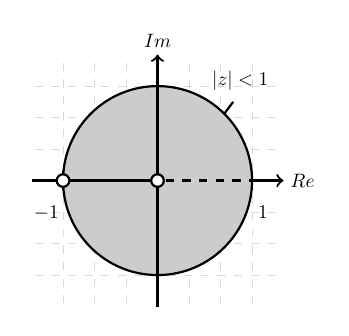
\begin{tikzpicture}[thick,scale=0.4, every node/.style={scale=0.7}]
\draw[help lines, color=gray!30, dashed] (-3.9,-3.9) grid (3.9,3.9);
\draw (2.12,2.12) -- (2.4,2.5);
 \fill[gray!40,even odd rule, dashed] (0,0) circle (3cm);
   \draw (0, 0) circle (3cm) node[above,xshift=1.5cm,yshift=1.5cm]{$|z|<1$};
\draw[thick] (3,-0.3) -- (3,0.3) node[below,xshift=0.2cm,yshift=-0.5cm]{$1$};
\draw[->, thick] (-4,0)--(4,0) node[right]{$Re$};
\draw[->, thick] (0,-4)--(0,4) node[above]{$Im$};
\draw[thick] (-3,-0.3) -- (-3,0.3) node[below,xshift=-0.3cm,yshift=-0.5cm]{$-1$};
\draw[gray!40, line width=0.5mm, dashed] (0,0)--(3,0);
 \filldraw[white, draw=black] (0,0) circle (0.2cm);
 \filldraw[white, draw=black] (-3,0) circle (0.2cm);
\end{tikzpicture}
\begin{tikzpicture}
\draw[color=white] (-1,0) rectangle (0.5,1);
\draw[thick,->] (-1,2) -- (0,2) node[above,xshift=-0.5cm]{$-z$};
\end{tikzpicture}
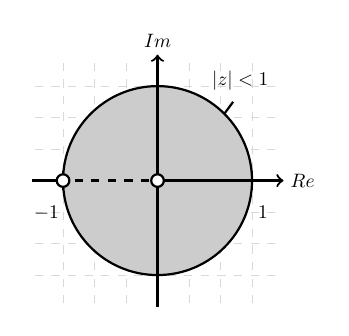
\begin{tikzpicture}[thick,scale=0.4, every node/.style={scale=0.7}]
\draw[help lines, color=gray!30, dashed] (-3.9,-3.9) grid (3.9,3.9);
\draw (2.12,2.12) -- (2.4,2.5);
 \fill[gray!40,even odd rule, dashed] (0,0) circle (3cm);
   \draw (0, 0) circle (3cm) node[above,xshift=1.5cm,yshift=1.5cm]{$|z|<1$};
\draw[thick] (3,-0.3) -- (3,0.3) node[below,xshift=0.2cm,yshift=-0.5cm]{$1$};
\draw[->, thick] (-4,0)--(4,0) node[right]{$Re$};
\draw[->, thick] (0,-4)--(0,4) node[above]{$Im$};
\draw[thick] (-3,-0.3) -- (-3,0.3) node[below,xshift=-0.3cm,yshift=-0.5cm]{$-1$};
\draw[gray!40, line width=0.5mm, dashed] (0,0)--(-3,0);
 \filldraw[white, draw=black] (0,0) circle (0.2cm);
 \filldraw[white, draw=black] (-3,0) circle (0.2cm);
\end{tikzpicture}
\begin{tikzpicture}
\draw[color=white] (-1,0) rectangle (0.5,1);
\draw[thick,->] (-1,2) -- (0,2) node[above,xshift=-0.5cm]{$w_1$};
\end{tikzpicture}
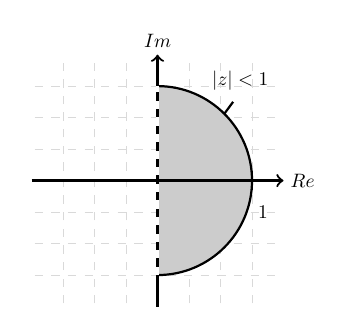
\begin{tikzpicture}[thick,scale=0.4, every node/.style={scale=0.7}]
\draw[help lines, color=gray!30, dashed] (-3.9,-3.9) grid (3.9,3.9);
\draw (2.12,2.12) -- (2.4,2.5);
 \fill[gray!40,even odd rule, dashed] (0,0) circle (3cm);
   \draw (0, 0) circle (3cm) node[above,xshift=1.5cm,yshift=1.5cm]{$|z|<1$};
\draw[thick] (3,-0.3) -- (3,0.3) node[below,xshift=0.2cm,yshift=-0.5cm]{$1$};
\draw[thick] (-3,-0.3) -- (-3,0.3) node[below,xshift=-0.3cm,yshift=-0.5cm]{$-1$};
\fill[white] (-4,-4) rectangle (0,4);
\draw[help lines, color=gray!30, dashed] (-3.9,-3.9) grid (0,3.9);
\draw[->, thick] (-4,0)--(4,0) node[right]{$Re$};
\draw[->, thick] (0,-4)--(0,4) node[above]{$Im$};
\draw[white,line width=0.4mm, dashed] (0,-3)--(0,3);
\end{tikzpicture}

\begin{tikzpicture}%[thick,scale=0.5, every node/.style={scale=0.6}]
\draw[thick,->] plot [smooth] coordinates {(3,0.6) (3,0) (-10,0) (-11,-1)} node[above,xshift=7cm,yshift=1cm]{$w_2$};
\end{tikzpicture}

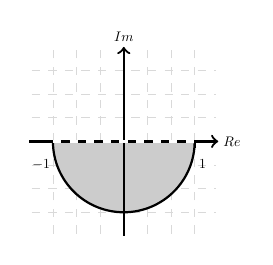
\begin{tikzpicture}[thick,scale=0.3, every node/.style={scale=0.5}]
\draw[help lines, color=gray!30, dashed] (-3.9,-3.9) grid (3.9,3.9);
\draw (2.12,2.12) -- (2.4,2.5);
 \fill[gray!40,even odd rule, dashed] (0,0) circle (3cm);
   \draw (0, 0) circle (3cm);
\draw[thick] (3,-0.3) -- (3,0.3) node[below,xshift=0.2cm,yshift=-0.5cm]{$1$};
\draw[thick] (-3,-0.3) -- (-3,0.3) node[below,xshift=-0.3cm,yshift=-0.5cm]{$-1$};
\fill[white] (-4,4) rectangle (4,0);
\draw[help lines, color=gray!30, dashed] (-3.9,3.9) grid (3.9,0);
\draw[->, thick] (-4,0)--(4,0) node[right]{$Re$};
\draw[->, thick] (0,-4)--(0,4) node[above]{$Im$};
\draw[white,line width=0.4mm, dashed] (-3,0)--(3,0);
\end{tikzpicture}
\begin{tikzpicture}
\draw[color=white] (-1,0) rectangle (0.5,1);
\draw[thick,->] (-1,2) -- (0,2) node[above,xshift=-0.5cm]{$T^{-1}$};
\end{tikzpicture}
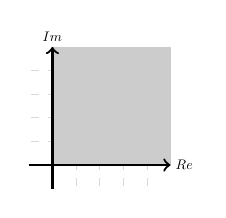
\begin{tikzpicture}[thick,scale=0.3, every node/.style={scale=0.5}]
\draw[help lines, color=gray!30, dashed] (-0.9,-0.9) grid (4.9,4.9);
 \fill[gray!40,even odd rule] (0,0) rectangle (5,5);
\draw[->, thick] (-1,0)--(5,0) node[right]{$Re$};
\draw[->, thick] (0,-1)--(0,5) node[above]{$Im$};
\end{tikzpicture}
\begin{tikzpicture}
\draw[color=white] (-1,0) rectangle (0.5,1);
\draw[thick,->] (-1,2) -- (0,2) node[above,xshift=-0.5cm]{$w_3$};
\end{tikzpicture}
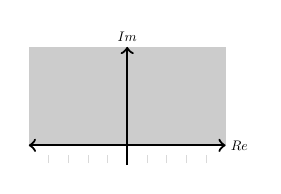
\begin{tikzpicture}[thick,scale=0.25, every node/.style={scale=0.5}]
\draw[help lines, color=gray!30, dashed] (-4.9,-0.9) grid (4.9,4.9);
 \fill[gray!40,even odd rule] (-5,0) rectangle (5,5);
\draw[<->, thick] (-5,0)--(5,0) node[right]{$Re$};
\draw[->, thick] (0,-1)--(0,5) node[above]{$Im$};
\end{tikzpicture}
\begin{tikzpicture}
\draw[color=white] (-1,0) rectangle (0.5,1);
\draw[thick,->] (-1,2) -- (0,2) node[above,xshift=-0.5cm]{$T$};
\end{tikzpicture}
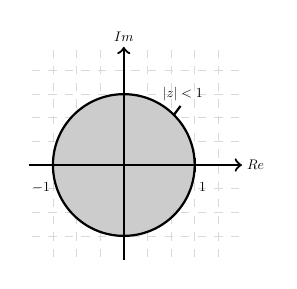
\begin{tikzpicture}[thick,scale=0.3, every node/.style={scale=0.5}]
\draw[help lines, color=gray!30, dashed] (-3.9,-3.9) grid (4.9,4.9);
\draw (2.12,2.12) -- (2.4,2.5);
 \fill[gray!40,even odd rule, dashed] (0,0) circle (3cm);
   \draw (0, 0) circle (3cm) node[above,xshift=1.5cm,yshift=1.5cm]{$|z|<1$};
\draw[thick] (3,-0.3) -- (3,0.3) node[below,xshift=0.2cm,yshift=-0.5cm]{$1$};
\draw[->, thick] (-4,0)--(5,0) node[right]{$Re$};
\draw[->, thick] (0,-4)--(0,5) node[above]{$Im$};
\draw[thick] (-3,-0.3) -- (-3,0.3) node[below,xshift=-0.3cm,yshift=-0.5cm]{$-1$};
\end{tikzpicture}
\end{center}
\end{solution}


\end{document}
